\documentclass{article}
\usepackage{spconf,amsmath,graphicx, cite, float, url}

% Example definitions.
% --------------------
\def\x{{\mathbf x}}
\def\L{{\cal L}}

% Title.
% ------
\title{Computer Security Report}
%
% Single address.
% ---------------
\name{Junsong Yang}
\address{School of Computer Science \\ University of Nottingham}
%
% For example:
% ------------
%\address{School\\
%	Department\\
%	Address}
%
% Two addresses (uncomment and modify for two-address case).
% ----------------------------------------------------------
%\twoauthors
%  {A. Author-one, B. Author-two\sthanks{Thanks to XYZ agency for funding.}}
%	{School A-B\\
%	Department A-B\\
%	Address A-B}
%  {C. Author-three, D. Author-four\sthanks{The fourth author performed the work
%	while at ...}}
%	{School C-D\\
%	Department C-D\\
%	Address C-D}
%
\begin{document}
%\ninept
%
\maketitle
%

\section{Passwords}
\label{sec:passwd}
In this section, the designed password and authentication policy will be proposed and justified.
First, the password policy will be explained in detail with additional authentication measures.
Then, mechanisms of storing passwords will be entailed.

\subsection{Password Policy}
As Gollmann \cite{GollmannDieter2011Cs/D}suggested, the overall security may be diminished 
if one security mechanism is overstated. Users tend to bypass the mechanism if it is too 
inappropriate for them to properly work with, hence the overall security of the system 
may be weakened. By considering that, the following password policies are proposed.

\subsubsection{Password Length}
This policy enforces the minimum number of character required to use as a valid password. 
Generally, the short the password, the more likely and easily to be cracked by brute-forcing.
Hence, by setting the minimum password length to ten, the difficulty for brute-forcing password 
cracking would be noticeably increased.

\subsubsection{Password Format}
This policy intended to accumulating the strength of a valid password by requiring what kind 
of character must be included in a password. By requiring the password to contain 
at least one lower and upper letter, one number, and one special character, combining with 
password length policy, the possibility of successful brute-force cracking would 
be significantly decreasing.

\subsubsection{Password Ageing}
This policy requires users to change their password periodically. The likelihood of password 
breaching would increase as time goes by, hence this is an appropriate approach to eliminate the 
risk of potential breaching.

\subsubsection{Password Use}
To further diminish the risk of potential password breaching over time, additional mechanism 
need to be employed to block users from using the same password twice. This policy is essential 
to assist the password ageing policy to fulfil its purpose.

\subsubsection{Password Choice}
The Dictionary attack is another approach frequently used for password cracking. The purpose of 
this policy is to prevent this attack. This problem can be addressed by preventing the user from 
using the password in public known dictionary.

\subsubsection{Login Attempts}
This policy is designed to reduce the risk of brute-force attack. By limiting the maximum number of 
failed login attempts the success rate of brute-force attack can be reduced significantly.

\subsection{Additional Authentication Measures}
Mechanisms must be implemented to address the repeated authentication problem. 
Between the time of check to time of use, user identity exploitation may occur as the 
authentication system does not keep track of what happened in between. 
Therefore, before some important actions like change password can be successfully performed, 
the user's identity needs to be checked again to ensure the action is legitimate.

\subsection{Storing Passwords}
As suggested by Gollmann, a password may be cached by browser\cite{GollmannDieter2011Cs/D}. Which 
suggests that storing raw password directly in the database is a bad practice. To maximise security, 
passwords should be hashed using one-way hash functions with salting and stretching approaches\cite{FergusonNiels2010Ce:d}.
Since hashing cannot be reversed, the original password will remain hidden.

\section{Firewalls}
\label{sec:firewalls}

Firewalls are software or hardware located between networks and filter potentially malicious 
packets from in and out traffic\cite{AndersonRoss1956-2008Se:a}.
Figure \ref{firewall} illustrates a network firewall which often stands between the local system and 
the internet compared to the host-based firewalls which located on individual machines. 
According to Gollmann, firewalls can also prevent unauthorised accesses of the internal-only services which 
block unnecessary or potentially dangerous access of external services from inside of the network\cite{GollmannDieter2011Cs/D}.

\begin{figure}[H]
  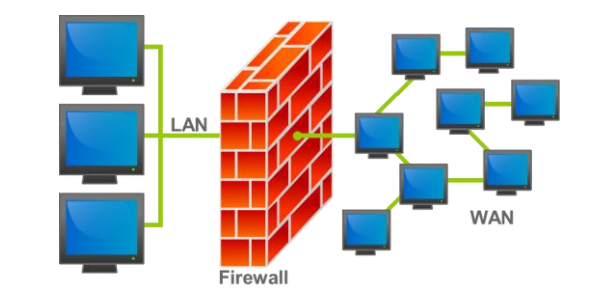
\includegraphics[width=8.5cm]{firewall}
  \caption{Network Firewall}
  \label{firewall}
\end{figure}

There several reasons that administrators may block port from normal traffic. As mentioned above, some services 
are only intended for internal access which suggests the necessity of blocking external access that 
may lead to security breaches. Another reason is that access external network from inside is also a potential 
breach in terms of the internal network as those ports are entrances to the network. 

As for the internal network, some internal traffic is unnecessary even potentially harmful. A peer-to-peer 
communication protocol BitTorrent, in this case, is most likely been blocked in some internal network.

\begin{figure}[H]
  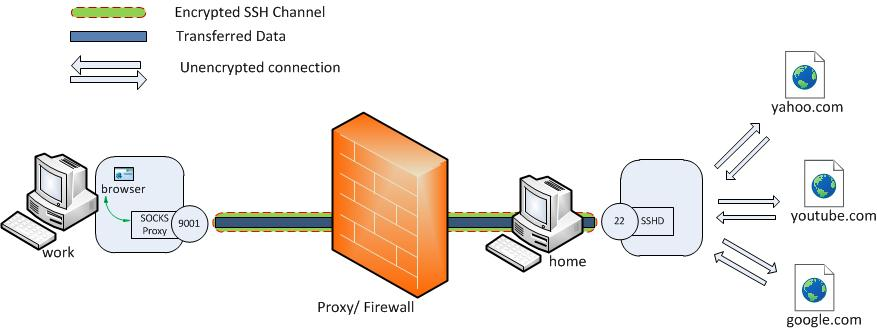
\includegraphics[width=8.5cm]{ssh}
  \caption{(a)SSH Tunnelling\cite{chamith_2012}}
  \label{ssh}
\end{figure}

Although some normal traffic is blocked or certain access rules are enforced by firewalls, there are ways 
to circumventing those rules and SSH tunnelling is one of them. 
SSH tunnelling is a way to establish an encrypted communication channel between two computers. In terms of 
bypassing the firewall rules, SSH tunnelling serves as a proxy. 
Figure \ref{ssh} shows how SSH tunnelling works in general.
Since the target server cannot be accessed directly, the request is first sent to the proxy 
server in the middle. Then the proxy server forwards the request to the target and returns the response 
back to the client. SSH tunnelling communicates with the proxy server by establishing an encrypted channel with 
the proxy server, and forward certain port on the local server to another port on the remote server.

\begin{figure}[H]
  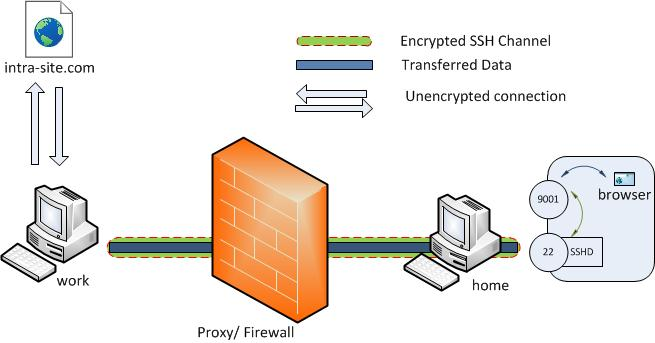
\includegraphics[width=8.5cm]{ssh1}
  \caption{(b) SSH Tunnelling\cite{chamith_2012}}
  \label{ssh1}
\end{figure}

Some usages of SSH tunnelling can be legitimate. As figure \ref{ssh1} demonstrates, the intra-site.com is 
a service only available from the internal network. By establishing the SSH tunnel with a machine inside the internal 
network, the internal services can be accessed from external. In this case, working remotely can be achieved. 
In fact, this approach is employed by most enterprises.

\begin{figure}[H]
  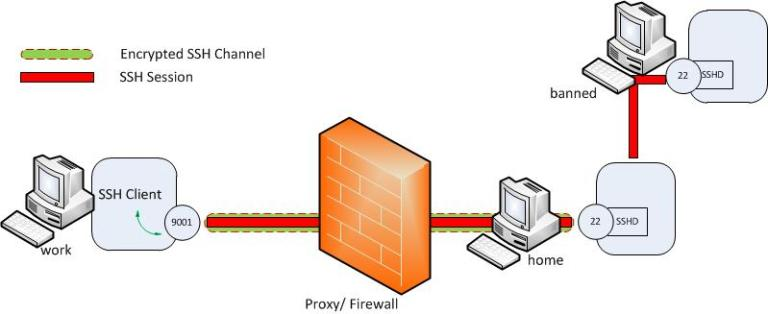
\includegraphics[width=8.5cm]{ssh2}
  \caption{(c) SSH Tunnelling \cite{chamith_2012}}
  \label{ssh2}
\end{figure}

Some usages of SSH tunnelling are disgraceful. In contrast to the example mentioned 
earlier, accessing blocked websites or services from the internal network, 
as figure \ref{ssh2}demonstrates, exposes the internal network to the whole Internet. 
In this case, the internal is exposed under risks that the firewall built to eliminate which directly 
invalidated the firewall. Hence, this way of using ssh tunnelling is considered disreputable. 

\section{Server Security}
\label{sec:serversec}

\subsection{Exploitation Process}
\begin{figure}[H]
  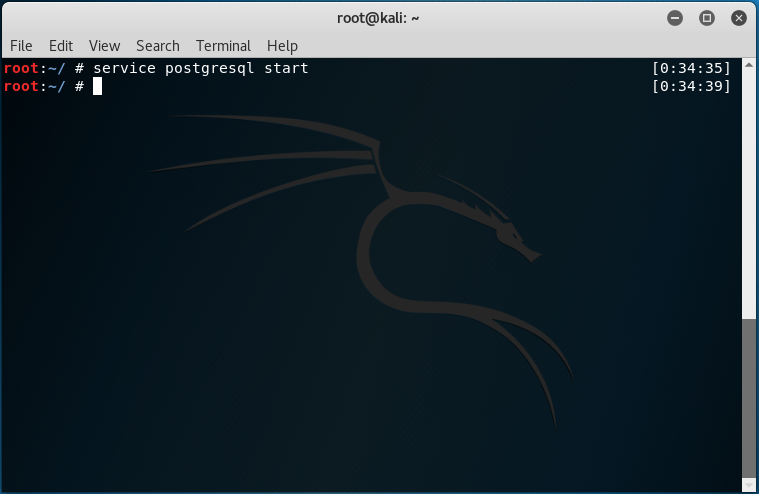
\includegraphics[width=8.5cm]{kali1}
  \caption{Sarting postgresql service}
  \label{kali1}
\end{figure}

Before the exploitation can begin, the necessary tools need to be prepared and initialised.
This exploitation requires Metasploit framework as backend and Armitage as front end. Since the 
Metasploit framework requires PostgreSQL database, as figure \ref{kali1} shows, 
the postgresql service needs to start first.

\begin{figure}[H]
  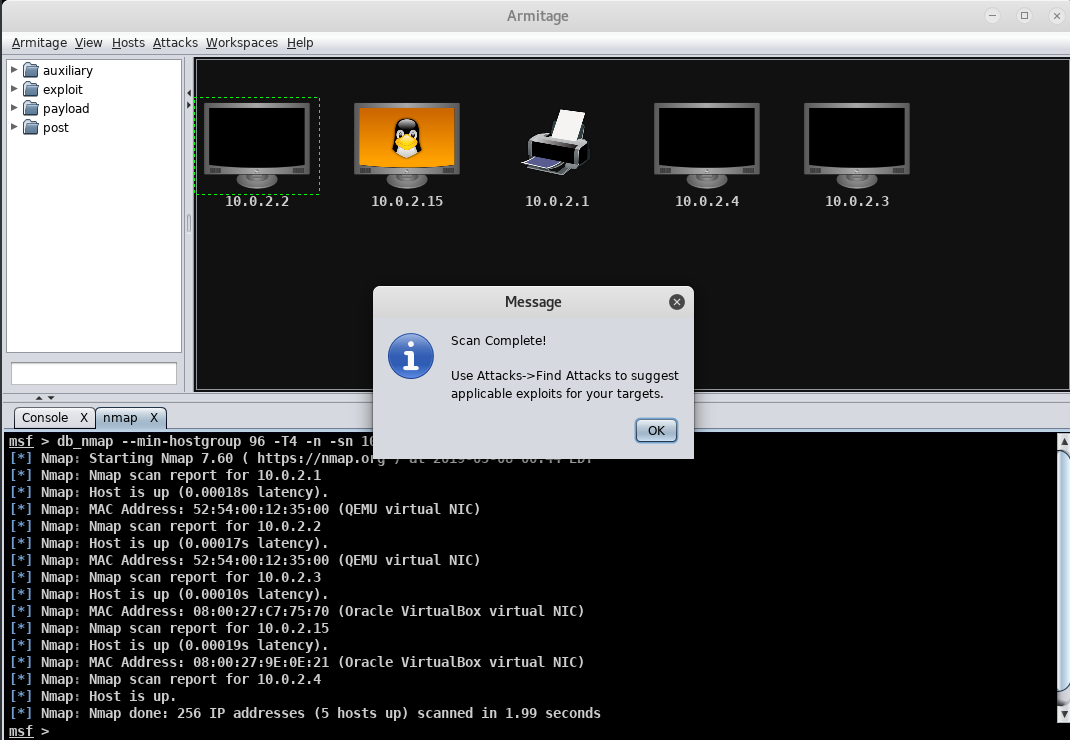
\includegraphics[width=8.5cm]{kali2}
  \caption{Ping Scan}
  \label{kali2}
\end{figure}

After the Armitage is successfully started, the first task is to detect all alive hosts within the 
same subnet using a ping scan provided by nmap. As figure \ref{kali2} shows, all alive host with IP address 
can be matched by 10.0.2.* are shown here.

\begin{figure}[H]
  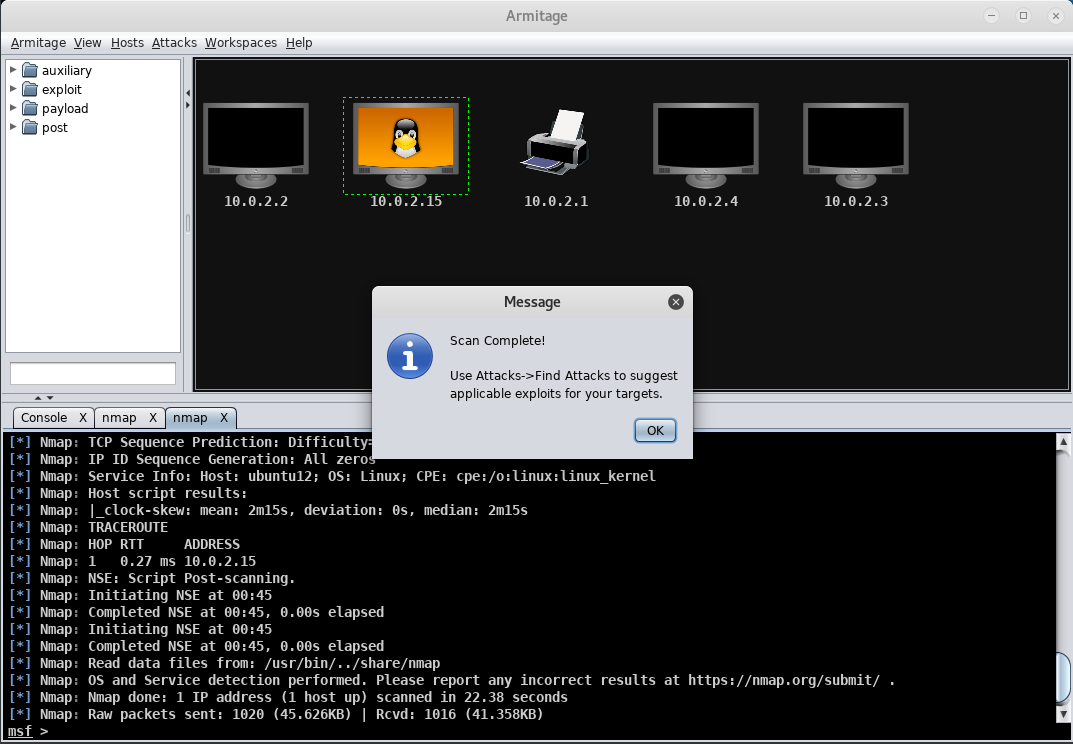
\includegraphics[width=8.5cm]{kali3}
  \caption{Intense Scan}
  \label{kali3}
\end{figure}

After all alive hosts are detected, the next step is to use intense scan provided by nmap to scan the 
target machine. As figure \ref{kali3} shows, system version, open ports, services running and their version 
can be detected during this step. This step is essential because it can provide crucial information 
for the attacker to determine where the security vulnerabilities exist and how to attack this machine.


\begin{figure}[H]
  \begin{minipage}[b]{1.0\linewidth}
    \centering
    \centerline{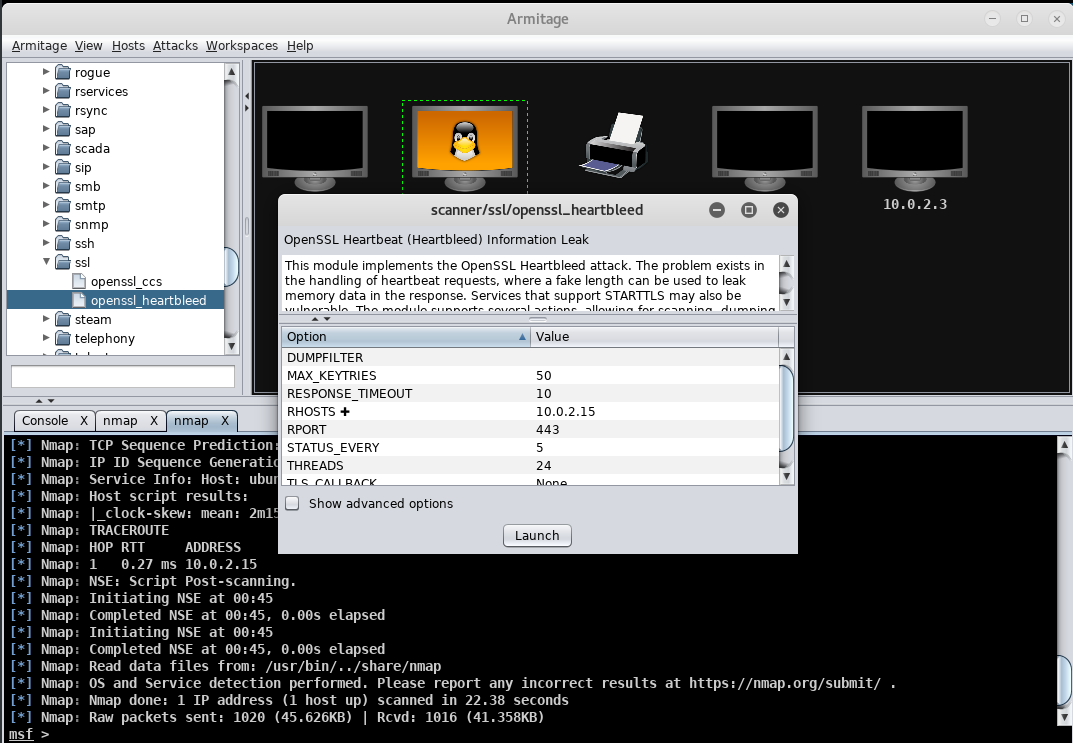
\includegraphics[width=8.5cm]{kali4}}
  %  \vspace{2.0cm}
    \centerline{(a) Heartbleed Exploitation}\medskip
  \end{minipage}

  \begin{minipage}[b]{.48\linewidth}
    \centering
    \centerline{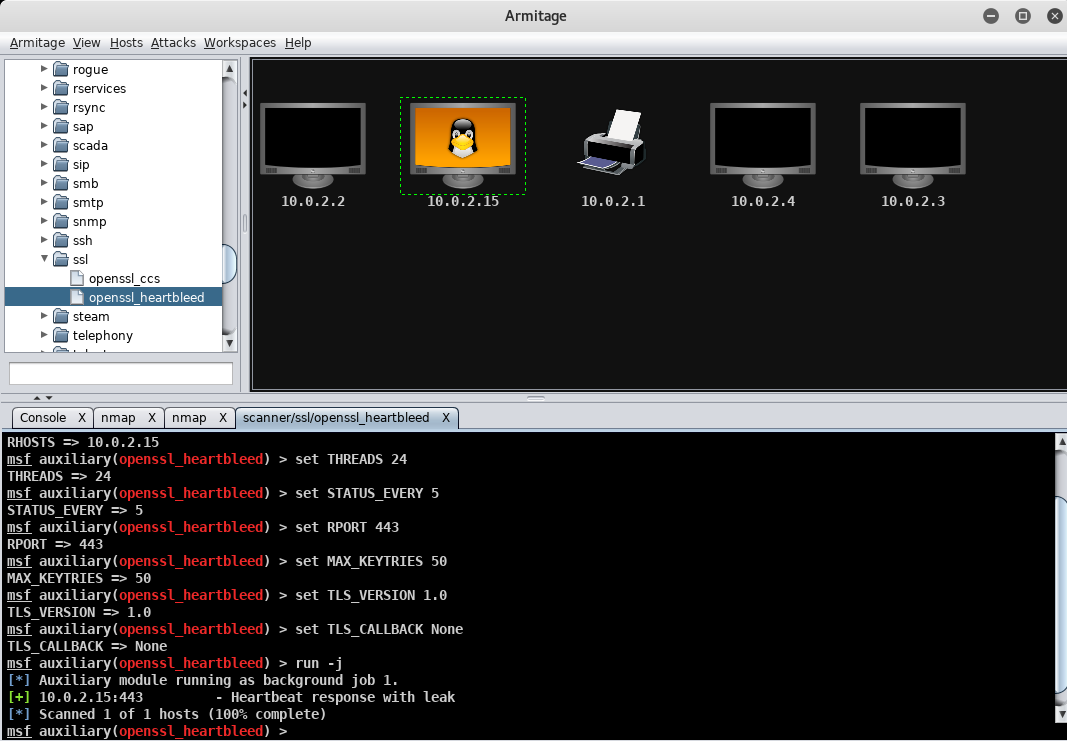
\includegraphics[width=4.0cm]{kali5}}
  %  \vspace{1.5cm}
    \centerline{(b) Heartbleed Exploitation}\medskip
  \end{minipage}
  \hfill
  \begin{minipage}[b]{0.48\linewidth}
    \centering
    \centerline{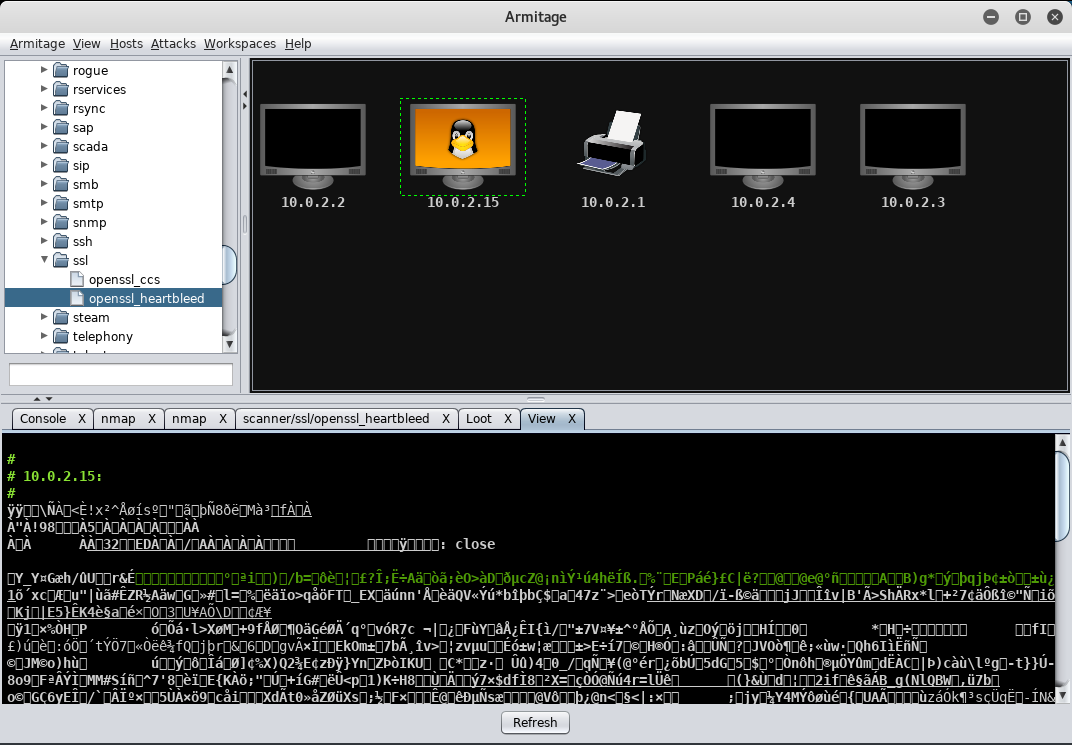
\includegraphics[width=4.0cm]{kali6}}
  %  \vspace{1.5cm}
    \centerline{(b) Heartbleed Exploitation}\medskip
  \end{minipage}
  %
  \caption{Heartbleed Exploitation Results.}
  \label{kali4-5-6}
  %
  \end{figure}

The next step as figure \ref{kali4-5-6} suggests, the heartbleed exploitation is carried out. This attack 
can be successfully carried out due to the host running a very old version of system and services where 
the heartbleed vulnerability still exists.

\begin{figure}[H]
  \begin{minipage}[b]{.48\linewidth}
    \centering
    \centerline{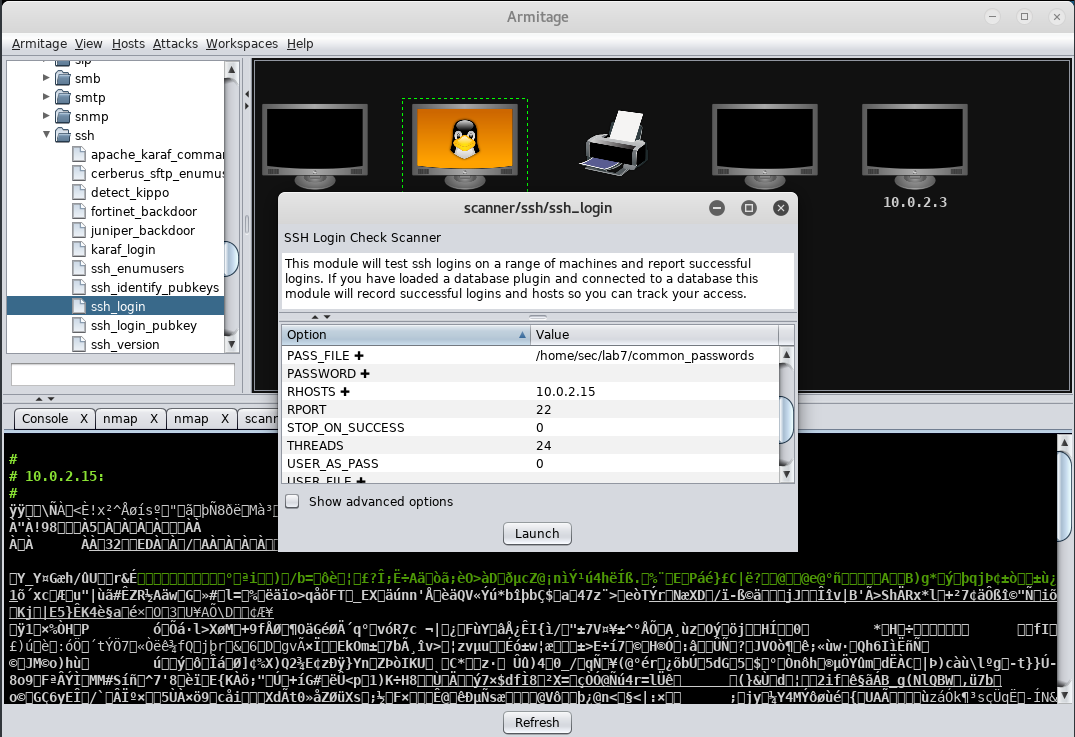
\includegraphics[width=4.0cm]{kali7}}
  %  \vspace{1.5cm}
    \centerline{(a) SSH Login Exploitation}\medskip
  \end{minipage}
  \hfill
  \begin{minipage}[b]{0.48\linewidth}
    \centering
    \centerline{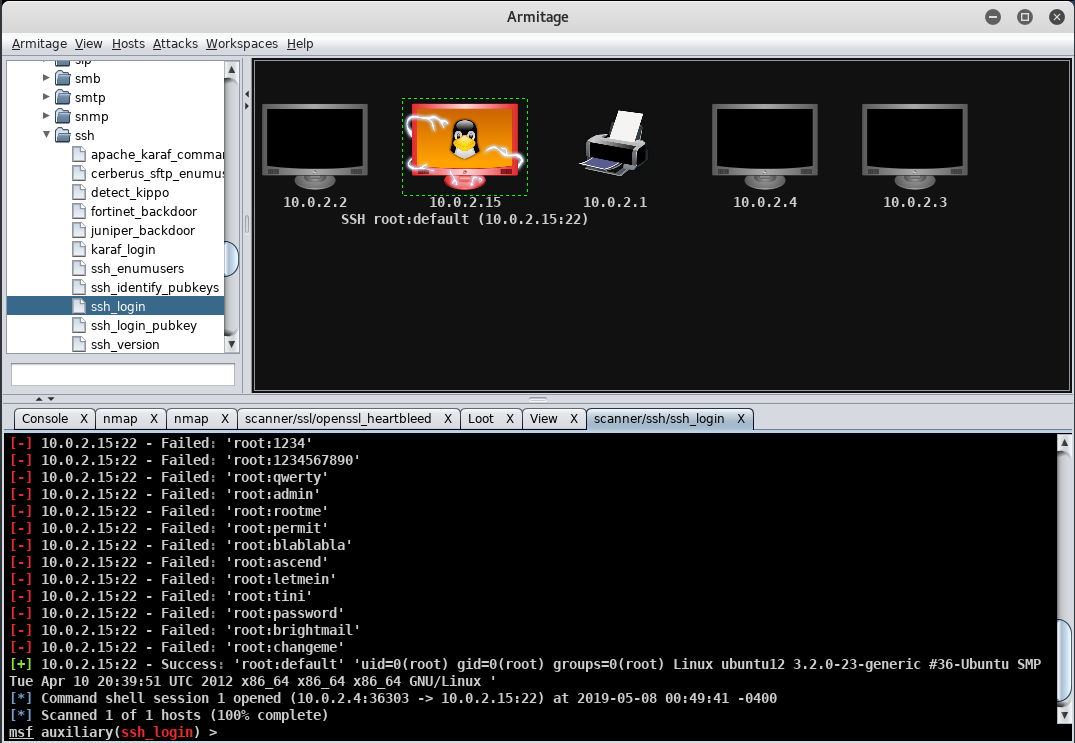
\includegraphics[width=4.0cm]{kali8}}
  %  \vspace{1.5cm}
    \centerline{(b) SSH Login Exploitation}\medskip
  \end{minipage}
  %
  \caption{SSH Login Exploitation Results.}
  \label{kali7-8}
  %
  \end{figure}
The next step is the most crucial one as the full access can be obtained after this step is successfully 
carried out. This step is to use provided password dictionary to carry out brute-force password cracking.
As figure \ref{kali7-8} shows, the root password was successfully acquired. Consequently, the full access to 
the host is now obtained.
Since no prior knowledge about the host is provided, with the success of root password cracking, 
all information required further can be obtained.

\begin{figure}[H]
  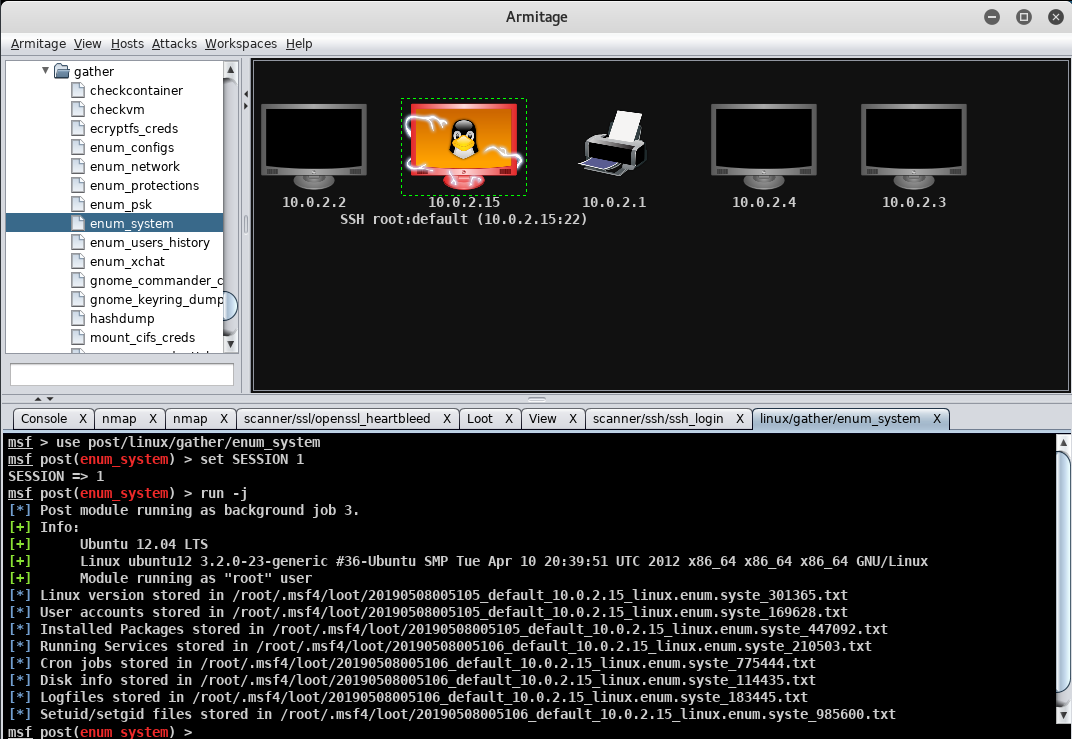
\includegraphics[width=8.5cm]{kali9}
  \caption{Gather System Information}
  \label{kali9}
\end{figure}

After the full access has been acquired, the last step of exploitation is to gather crucial system information 
like packages installed and their version, all currently running services, system information and kernel version, 
user list, and service list.
As shown in figure \ref{kali9}, all this information is stored in text files.


\subsection{Security Fixes}
As mentioned in the previous section, the target host needs to be detected first before any exploitation can begin.
In addition, the detection process was using the ping scan provided by nmap. Therefore, the first security vulnerability 
need to be fixed is to prevent the machine from being detected. In this case, a firewall rule was added to the Ubuntu 
machine.

\begin{figure}[H]
  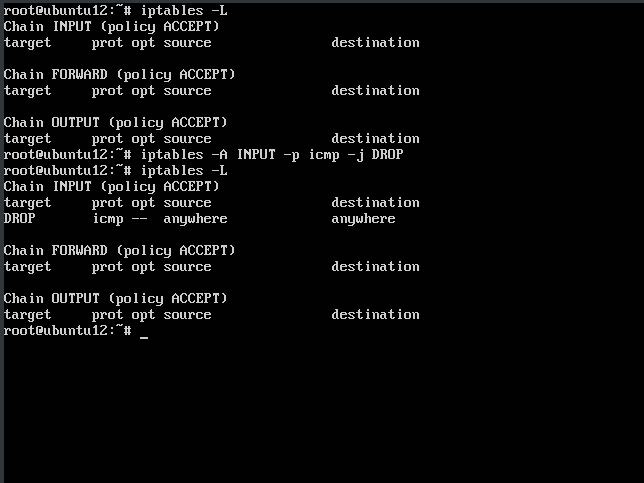
\includegraphics[width=8.5cm]{ubuntu4}
  \caption{IPTables}
  \label{ubuntu4}
\end{figure}

As shown in figure \ref{ubuntu4}, the default firewall is quite permissive and allow any traffic by default. 
By adding a rule, all packet sent by ping action will be dropped. 

\begin{figure}[H]
  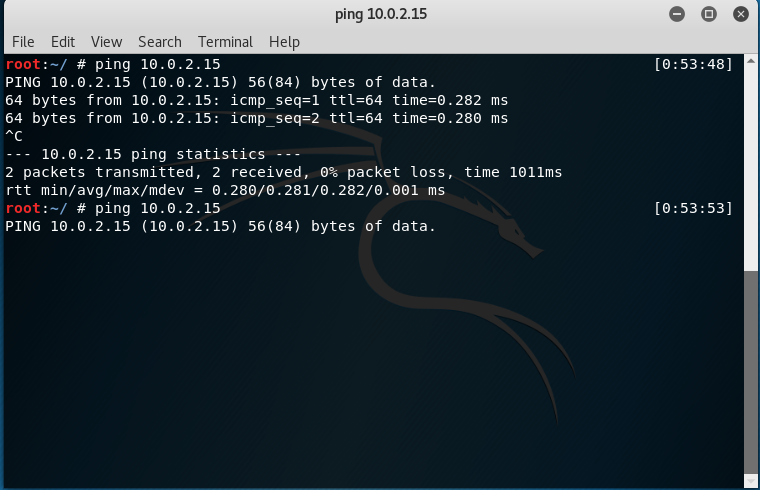
\includegraphics[width=8.5cm]{kali10}
  \caption{IPTables Effect}
  \label{kali10}
\end{figure}

Figure \ref{kali10} shows the immediate effect after this rule being enforced. The first attempt suggests the firewall 
with default settings. It is obvious that the target host was responding as normal which is a positive 
confirmation of the target state. After the firewall being updated, the target stopped responding to the ping request. 
The target machine is either confirm nor deny, the ping requests. Hence, the attacker cannot determine the state of 
the target host. Therefore, in this case, the attacker may turn to the targets that return a positive response. 
Technically, other approaches can be employed to detect the state of the target, but psychologically this method is 
quite like effective.

\begin{figure}[H]
  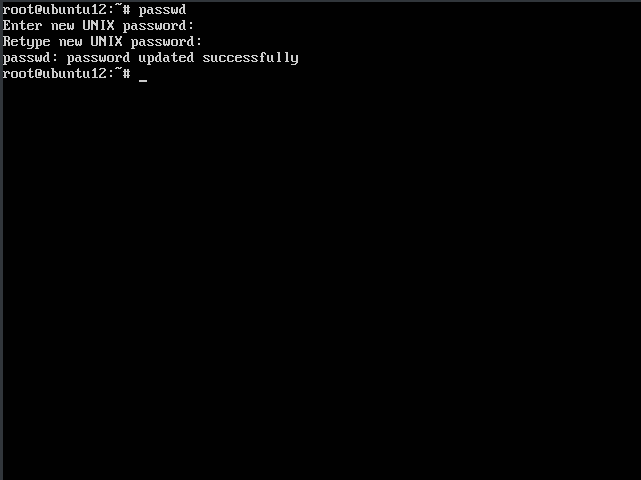
\includegraphics[width=8.5cm]{ubuntu8}
  \caption{Changing Password}
  \label{ubuntu8}
\end{figure}

The second crucial step of exploiting this machine is to crack the root password by brute-forcing. 
Therefore, the first step of fixing this vulnerability, as figure \ref{ubuntu8} shows, is to change the current password into a strong one which 
will significantly increase the cost of brute-forcing. Due to the time constraint, password checking against 
publicly known dictionaries is yet to be implemented.

\begin{figure}[H]
  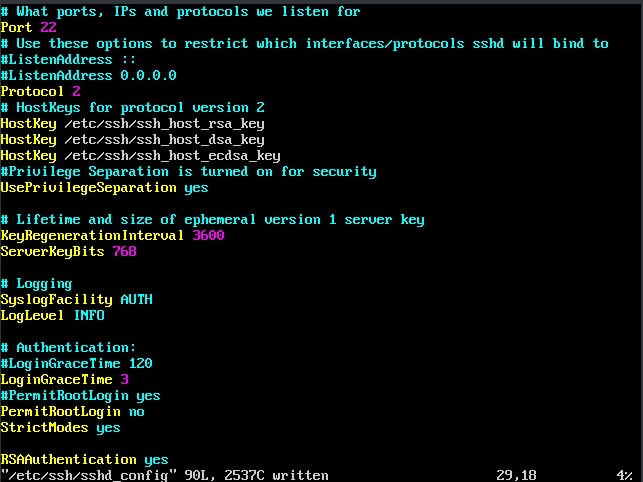
\includegraphics[width=8.5cm]{ubuntu6}
  \caption{Changing Password}
  \label{ubuntu6}
\end{figure}

Another factor that allows the brute-force cracking to continue is the maximum number of login attempts allowed 
was too big. As figure \ref{ubuntu6} depicts, the default setting was 120. This issue can be easily fixed by changing 
this number to a small one(in this case, it was set to three).

By default, almost no password policy was enforced. Other than policies implemented earlier, all of the password policies 
proposed for question one should be employed given enough time.

In the Unix system, the root is the most powerful user as it has permissions to do anything. Therefore, it would be a disaster for 
systems to have root password breaching. The ultimate solution to address this issue is to forbid user login as root 
as shown in figure \ref{ubuntu6}. Furthermore, the only solution to prevent password leaking for all user is to 
prevent users from login using the password.

\begin{figure}[H]
  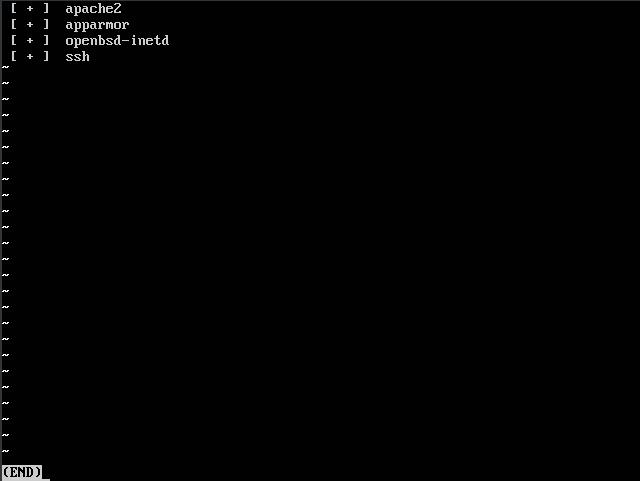
\includegraphics[width=8.5cm]{ubuntu3}
  \caption{Running Service List}
  \label{ubuntu3}
\end{figure}
Figure \ref{ubuntu3} shows the list of running services. Telnet and ftp service are provided by openbsd-inetd service 
which should never be used as they transferring all information in plain text without any encryption.

Due to the time constraint, all packages in the Ubuntu system are still in default version. Almost all packages 
alongside the kernel should be updated as they are hopelessly outdated. Many security breaches that should be fixed 
for a long time may still exist in this system.



% To start a new column (but not a new page) and help balance the last-page
% column length use \vfill\pagebreak.
% -------------------------------------------------------------------------

\vfill
\pagebreak

\vfill
\pagebreak

\bibliographystyle{IEEEbib}
\bibliography{bibtex}

\end{document}
